\documentclass[12pt,titlepage]{article}

\usepackage{geometry}
\geometry{
    a4paper,
    total={210mm,297mm},
    left=20mm,
    right=20mm,
    top=20mm,
    bottom=20mm,
}

	
\usepackage[]{subcaption}

\usepackage{pdflscape}

% Polski
\usepackage[]{polski} 
\usepackage[polish]{babel}

%do tabel
\usepackage{multirow}

% Pierwszy akapit - wcięty
\usepackage[]{indentfirst}

% Matematyka
\usepackage[]{amsfonts}

\usepackage[]{amsmath}

% Formatowanie
\usepackage{ragged2e}

% Tytuły sekcji
\usepackage{titlesec}
%\titleformat{\section}[block]{\Large\bfseries}{}{1em}{}

% <=
\usepackage{amssymb}

% eps
\usepackage{graphicx}
% \usepackage{subfigure}

% Tabele
\usepackage{array}

\usepackage[style=czech]{csquotes}

\renewcommand*{\thesubsubsection}{}

\usepackage{hyperref}
\hypersetup{
    colorlinks,
    citecolor=black,
    filecolor=black,
    linkcolor=black,
    urlcolor=black
}

\usepackage[numbered]{matlab-prettifier}
\lstset{
    literate={ą}{{\k{a}}}1
    {Ą}{{\k{A}}}1
    {ę}{{\k{e}}}1
    {Ę}{{\k{E}}}1
    {ó}{{\'o}}1
    {Ó}{{\'O}}1
    {ś}{{\'s}}1
    {Ś}{{\'S}}1
    {ł}{{\l{}}}1
    {Ł}{{\L{}}}1
    {ż}{{\.z}}1
    {Ż}{{\.Z}}1
    {ź}{{\'z}}1
    {Ź}{{\'Z}}1
    {ć}{{\'c}}1
    {Ć}{{\'C}}1
    {ń}{{\'n}}1
    {Ń}{{\'N}}1
}

\title{

\includegraphics[scale=0.75]{img/politechnika_sl_logo_bw_poziom_pl.eps}\\
\textbf{Wydział Automatyki, Elektroniki\\
i Informatyki}\\
\vspace*{1cm}
Technologie aplikacji internetowych \\ Projekt \\ PairPay

\vspace*{5cm}
}
\author{
Natalia Stręk,\\
Jakub Kula,\\
Paweł Wójtowicz
} 
\date{Gliwice 2024}

\begin{document}

\maketitle
\newpage
\section{Przedstawienie pomysłu na projektu}

Aplikacja do zarządzania wydatkami została zaprojektowana z myślą o osobach regularnie dzielących się kosztami, na przykład podczas wspólnych podróży, zakupów czy spotkań towarzyskich. Jej głównym celem jest uproszczenie procesu rejestrowania, monitorowania i rozliczania wydatków w grupach, co umożliwia efektywne zarządzanie finansami oraz minimalizuje ryzyko nieporozumień związanych z podziałem kosztów.\\

Użytkownicy mogą zarejestrować się i zalogować do systemu, uzyskując tym samym dostęp do chronionych funkcji aplikacji. Aplikacja pozwala na tworzenie nowych rachunków, do których można dodawać wydatki oraz uczestników, a następnie automatycznie dzieli koszty na podstawie wprowadzonych danych. Dzięki funkcji skanowania paragonów użytkownicy mogą łatwo importować informacje o wydatkach, eliminując konieczność ręcznego wprowadzania szczegółów.\\

Aplikacja oferuje także możliwość edytowania i usuwania rachunków oraz przeglądania historii wydatków, co zapewnia użytkownikom pełną kontrolę nad ich finansami. Dodatkowo, opcje filtrowania i sortowania rachunków, a także etykietowania wydatków, zwiększają użyteczność aplikacji, umożliwiając łatwe odnalezienie oraz zarządzanie danymi.\\

Wszystkie te funkcje sprawiają, że aplikacja jest nieocenionym narzędziem dla osób pragnących efektywnie zarządzać swoimi wydatkami, oszczędzając przy tym czas i minimalizując ryzyko błędów przy podziale kosztów.

\section{User Story}
\subsection{Para dzieląca się wydatkami}
Para, która mieszka razem, często robi wspólne zakupy. Zazwyczaj jedna osoba wybiera się na większe zakupy spożywcze, a druga później zwraca swoją część kosztów. Niestety, czasami pojawiają się problemy z ustaleniem, ile dokładnie każdy powinien zapłacić, bo paragonów przybywa, a nie zawsze jest czas, by od razu je podsumować. Dzięki aplikacji pariPay można na bieżąco dodawać wydatki do wspólnego rachunku i nie martwić się o szczegóły. 
\subsection{Rozliczenie rachunku w restauracji}
Grupa znajomych wybrała się na kolację do ulubionej restauracji. Po posiłku jedna osoba zdecydowała się opłacić cały rachunek. Zamiast przeliczać, kto co zamówił i ile powinien zapłacić, skorzystano z aplikacji pariPay. Wszystkie pozycje z paragonu zostały wprowadzone, przypisane do odpowiednich osób, a jednym kliknięciem wysłano znajomym wiadomość o rozliczeniu. Każdy może teraz bez problemu opłacić swoją część rachunku bez nieporozumień i przeliczania.
\subsection{Składka na imprezę z różnym rozliczaniem kosztów}
Podczas organizacji domowej imprezy grupa znajomych ustaliła, że złożą się na jedzenie i przekąski, a jedna osoba zadba o zakup napojów alkoholowych. Po imprezie pojawiła się potrzeba rozliczenia kosztów, jednak nie wszyscy spożywali alkohol, więc podział nie mógł być równy. W takim przypadku skorzystano z aplikacji pariPay, która pozwala na wprowadzenie wszystkich wydatków do wspólnego rachunku i precyzyjne przypisanie kosztów – np. pełne rozliczenie napojów alkoholowych tylko do tych, którzy je spożywali. Dzięki temu rachunek został podzielony sprawiedliwie, uwzględniając rzeczywiste wydatki każdej osoby.

\section{Specyfikacja wymagań aplikacji}
    \begin{table}[!h]
        \centering
        \resizebox{\textwidth}{!}{
            \begin{tabular}{|c|l|p{0.35\textwidth}|p{0.55\textwidth}|}
                \hline
                \textbf{Nr} & \textbf{Nazwa} & \textbf{Opis} & \textbf{Kryterium odbioru} \\ \hline
                \textbf{F\_1} & Logowanie i rejestracja & 
                Użytkownik może zakładać konto oraz logować się na nie. &
                System musi umożliwiać rejestrację, logowanie, oraz uzyskanie dostępu do chronionych funkcji aplikacji. Każda interakcja z chronionymi zasobami wymaga sprawdzenia tożsamości. Użytkownik musi także móc się wylogować, co kończy sesję i blokuje dostęp do zasobów. \\ \hline
                \textbf{F\_2} & Tworzenie nowego rachunku & 
                Użytkownik może tworzyć nowy rachunek, dodawać przedmioty oraz uczestników do podziału kosztów. &
                Użytkownik musi móc wprowadzić nazwę rachunku, dodać uczestników i szczegóły, a następnie zapisać rachunek. Rachunek musi być widoczny dla wszystkich dodanych uczestników. System musi poprawnie zapisywać dane rachunku oraz umożliwiać ich przeglądanie i edycję. \\ \hline
                \textbf{F\_3} & Dodanie nowych wydatków & 
                Aplikacja umożliwia dodawanie nowych wydatków do istniejących rachunków. &
                Użytkownik musi móc wprowadzić szczegóły wydatku, takie jak kwota, opis oraz przypisanie do uczestników. System musi aktualizować saldo rachunku i widok wydatków, a także potwierdzić dodanie wydatku. \\ \hline
                \textbf{F\_4} & Automatyczny podział kosztów & 
                Aplikacja automatycznie dzieli koszty między użytkowników. &
                System musi poprawnie obliczać i wyświetlać udział każdej osoby w rachunku, bazując na wydatkach oraz przypisanych uczestnikach. Użytkownik może wybrać metodę podziału (np. równy lub według udziałów) i otrzymać podsumowanie. System aktualizuje informacje po dodaniu nowych wydatków. \\ \hline
                \textbf{F\_5} & Automatyczne odczytywanie paragonów & 
                Aplikacja umożliwia wgranie zdjęcia paragonu, z którego odczytywane są informacje o kosztach. &
                System musi poprawnie rozpoznać i wydobyć kluczowe dane z paragonu (datę, kwotę, szczegóły wydatków). Użytkownik może przesłać obraz paragonu, a system zapisze te informacje w rachunku, potwierdzając ich dodanie. \\ \hline
                \textbf{F\_6} & Tworzenie grup znajomych & 
                Możliwość zapisywania grup osób, z którymi użytkownik często współdzieli rachunki. &
                Użytkownik może tworzyć grupy, nadając im nazwy i dodając członków z listy znajomych. System umożliwia edytowanie, usuwanie grup, oraz wyświetla wszystkie grupy użytkownika. \\ \hline
                \textbf{F\_7} & Edytowanie i usuwanie rachunku & 
                Aplikacja umożliwia edytowanie oraz usuwanie rachunków. &
                Użytkownik może edytować szczegóły rachunku (nazwa, uczestnicy, wydatki). System zapisuje zmiany i aktualizuje informacje, a także umożliwia usunięcie rachunku z odpowiednim potwierdzeniem i powiadomieniem uczestników. \\ \hline
                \textbf{F\_8} & Historia rachunków & 
                Aplikacja zapisuje poprzednie rachunki, umożliwiając przeglądanie historii. &
                Użytkownik ma możliwość wyświetlania listy wcześniejszych rachunków, wraz z informacjami o nazwie, dacie oraz uczestnikach, a także przeglądania szczegółów każdego rachunku. \\ \hline
                \textbf{F\_9} & Filtrowanie i sortowanie rachunków & 
                Aplikacja umożliwia filtrowanie i sortowanie rachunków według różnych kryteriów. &
                Użytkownik może stosować różne filtry, takie jak data, uczestnicy, kwota. System aktualizuje widok rachunków zgodnie z wybranymi kryteriami, umożliwiając sortowanie według wybranych parametrów. \\ \hline
                \textbf{F\_10} & Etykietowanie rachunków & 
                Aplikacja umożliwia przypisanie etykiet do wydatków, określających ich typ (np. rozrywka, transport, dom). &
                System musi umożliwiać łatwe przypisywanie i przeglądanie etykiet, co ułatwia klasyfikację wydatków w rachunkach. \\ \hline
                \textbf{F\_11} & Panel administracji & 
                Administrator może monitorować różne statystyki za pośrednictwem aplikacji typu ilość użytkowników, grup. & System powinien umożliwiać wgląd tylko autoryzowanym użytkownikom i w prawdiłowy sposób wyświetlać informację.
                System umożliwia na  \\ \hline
                \textbf{F\_12} & Obsługa płatności & Obsługa rozliczeń rachunków w grupach użytkowników
                 &    \\ \hline
            \end{tabular}
        }
        \caption{Opis funkcjonalności aplikacji oraz kryteriów odbioru}
        \label{tab:funkcjonalnosci}
    \end{table}
    
    \newpage
    \begin{table}[!h]
        \centering
        \renewcommand{\arraystretch}{1.3} 
        \resizebox{\textwidth}{!}{
            \begin{tabular}{|c|l|p{0.7\textwidth}|}
                \hline
                \textbf{Kod}    & \textbf{Nazwa}       & \textbf{Opis} \\ \hline
                \textbf{NF\_1}  & Wydajność            & Aplikacja powinna ładować strony i przeprowadzać operacje w sposób płynny, zapewniając komfortowe doświadczenie użytkownika. \\ \hline
                \textbf{NF\_2}  & Bezpieczeństwo       & 
                \begin{itemize}
                    \item Bezpieczne przechowywanie wrażliwych danych użytkowników poprzez szyfrowanie.
                    \item Ochrona przed nieuprawnionym dostępem (ochrona przed atakami typu SQL injection, autentykacja i autoryzacja) 
                    \item Ochrona zasobów poprzez ścieżki kontrolowane (panel administracji) oraz autoryzację za pomocą tokenów
                \end{itemize}
                \\ \hline
                \textbf{NF\_3}  & Użyteczność          & Interfejs użytkownika powinien być prosty i intuicyjny, zawierając jasne instrukcje dotyczące dodawania rachunków, etykietowania i podziału kosztów, aby zminimalizować krzywą uczenia się dla nowych użytkowników. \\ \hline
                \textbf{NF\_4}  & Dokumentacja         & Aplikacja powinna posiadać szczegółową dokumentację zarówno dla użytkowników, jak i administratorów, opisującą wszystkie funkcje oraz procedury użytkowania. \\ \hline
                \textbf{NF\_5}  & Kompatybilność         & Aplikacja musi działać poprawnie na większości popularnych przeglądarek internetowych, a także na urządzeniach o różnej rozdzielczości ekranu. \\ \hline
                \textbf{NF\_6}  & Intuicyjność obsługi aplikacji         & 
                Aplikacja powinna mieć prosty i intuicyjny interfejs, umożliwiający łatwe korzystanie użytkownikom w różnym wieku. \\ \hline
            \end{tabular}
        }
        \caption{Opis wymagań niefunkcjonalnych aplikacji}
        \label{tab:non-functional-requirements}
    \end{table}
        
    


\newpage
\section{Skala MoSCow}
    
\begin{table}[ht]
    \centering
    \renewcommand{\arraystretch}{1.3} 
    \begin{tabular}{|c|c|}
        \hline
        \textbf{Funkcjonalność} & \textbf{Skala MoSCoW} \\ \hline
        \textbf{F\_1}           & Must                  \\ \hline
        \textbf{F\_2}           & Must                  \\ \hline
        \textbf{F\_3}           & Must                  \\ \hline
        \textbf{F\_4}           & Should                \\ \hline
        \textbf{F\_5}           & Could                 \\ \hline
        \textbf{F\_6}           & Should                \\ \hline
        \textbf{F\_7}           & Should                \\ \hline
        \textbf{F\_8}           & Should                \\ \hline
        \textbf{F\_9}           & Could                 \\ \hline
        \textbf{F\_10}          & Could                 \\ \hline
        \textbf{F\_11}          & Could                 \\ \hline
        \textbf{F\_12}          & Won't                 \\ \hline
        \textbf{NF\_1}          & Must                  \\ \hline
        \textbf{NF\_2}          & Must                  \\ \hline
        \textbf{NF\_3}          & Should                \\ \hline
        \textbf{NF\_4}          & Could                 \\ \hline
        \textbf{NF\_5}          & Must                \\ \hline
        \textbf{NF\_6}          & Should                 \\ \hline
    \end{tabular}
    \caption{Klasyfikacja funkcjonalności według skali MoSCoW}
    \label{tab:moscow-classification}
\end{table}

\newpage

\section{Diagram przypadków użycia}
\begin{figure}[h]
    \centering
    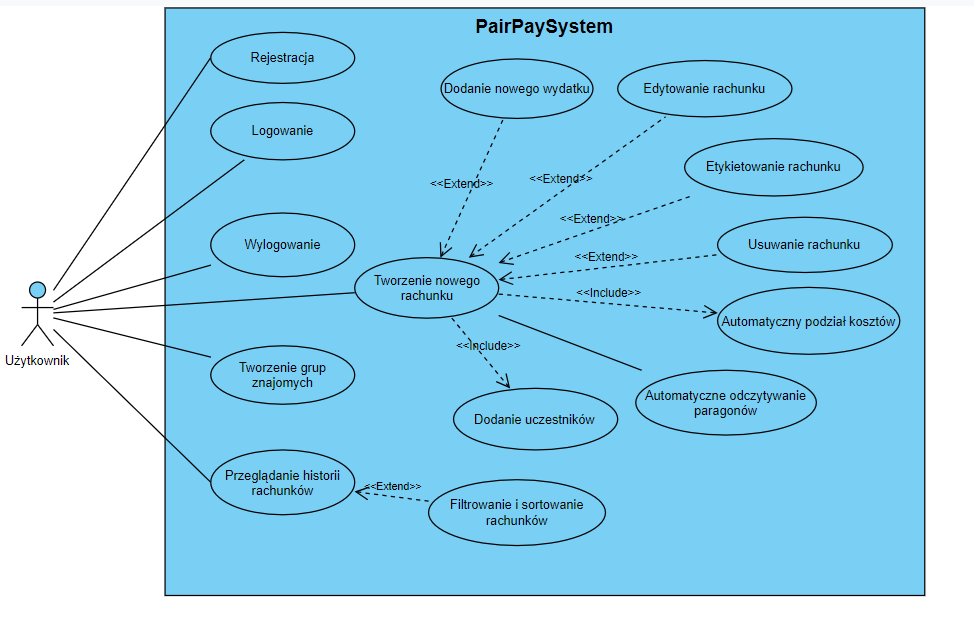
\includegraphics[width=1\textwidth]{img/UserDiagram.png}
    \caption{Diagram przypadków użycia}
    \label{fig:mesh1}
\end{figure}


\newpage
\section{Komponenty systemu}
\subsection{Backend - REST API}
\begin{itemize}
    \item Technologie: Python z frameworkiem Flask
    \item Uzasadnienie: Flask jest oparty o język Python, co umożliwia korzystanie z jego licznych zalet. To lekki framework, który umożliwia szybkie tworzenie aplikacji backendowych. Daje pełną elastyczność w projektowaniu różnych rozwiązań. Jest idealny do tworzenia REST API i umożliwia łatwą integrację między frontendem a backendem. Kolejnym ważym argumentem jest jego wsparcie dla OAuth, co pozwala zapewnić bezpieczne logowanie i autoryzację użytkowników. Kolejnym ważnym aspektem jest to, że Flask świetnie wsółdziała z takimi bibliotekami jak SQLAlchemy czy Tortoise ORM, co znacznie upraszcza operacje na bazie danych i tworzenie powiązań między tabelami. Ogromną zaletą Flaska jest również wsparcie społeczności i rozbudowana dokumentacja, która umożliwi szybkie znalezienie rozwiązań na różne problemy.
\end{itemize}

\subsection{Frontend}
\begin{itemize}
    \item Technologie: TypeScript z frameworkiem React
    \item Uzasadnienie: React to popularna biblioteka do budowy interfejsów użytkownika, która umożliwia tworzenie dynamicznych i responsywnych aplikacji webowych. Dzięki zastosowaniu komponentów, zarządzanie stanem aplikacji staje się prostsze, a ponowne wykorzystanie kodu znacząco przyspiesza proces developmentu. Wirtualny DOM, oferowany przez React, zwiększa wydajność aplikacji, umożliwiając szybkie aktualizacje interfejsu użytkownika bez nadmiernego obciążania przeglądarki. Dodatkowo, dostępność licznych bibliotek z gotowymi komponentami UI, takich jak NextUI czy Shadcn, umożliwia szybkie i efektywne tworzenie elementów interfejsu, co przyspiesza rozwój aplikacji.
\end{itemize}

\subsection{Baza danych}
\begin{itemize}
    \item Technologie: PostgreSQL
    \item Uzasadnienie: PostgreSQL jest relacyjną bazą danych, która jest wydajna oraz dobrze skalowalna, potrafi obsłużyć duże ilości danych i skomplikowane zapytania. Posiada również wsparcie dla JSON, co pozwala na przechowywanie danych nieustrukturyzowanych. Kolejnym ważnym aspektem jest aktywna społeczność, co powoduje, że jest wiele zasobów oraz dokumentacji w przypadku pojawienia się jakiegoś problemu. Dodatkowo, PostgreSQL oferuje zaawansowane funkcje bezpieczeństwa, takie jak wielopoziomowe uwierzytelnianie, kontrola dostępu oraz szyfrowanie danych. Te mechanizmy zabezpieczeń chronią przed nieautoryzowanym dostępem i utratą danych, co jest kluczowe w kontekście aplikacji, które przechowują wrażliwe informacje finansowe.
\end{itemize}

\subsection{Development}
\begin{itemize}
    \item Technologie: Git (GitHub) oraz CI/CD z Dockerem (GitHub Actions) ?? do ci/cd mozna napisac ze umozliwia na automatyczne puszczanie testow jednostkowych czy e2e, na sprawdzanie kodu zastosowanie jakis formaterow kodu, budowanie obrazow dockerowych itp... ??TODO docker-compose i zastanowic sie czy to dac
    \item Uzasadnienie: Umożliwiaja monitorowanie zmian w kodzie, co pozwala na łatwe śledzenie postępów w projekcie oraz ułatwia pracę zespołową poprzez wykorzystanie branchy do izolacji pracy nad różnymi funkcjonalnościami aplikacji, co zmniejsza ryzyko konfliktów w kodzie. GitHub Actions, jako narzędzie wbudowane w GitHub, automatyzuje procesy \\ CI/CD bezpośrednio w repozytoriach i oferuje elastyczność w definiowaniu potoków \\ CI/CD w plikach YAML. 
\end{itemize}


\subsection{Diagram komponentów}

\begin{figure}[!h]
    \centering
    \includegraphics[width=1\textwidth]{img/Digram_komponentów.pdf}
    \caption{Diagram komponentów}
    \label{fig:mesh1}
\end{figure}
\newpage
\subsection{Diagram sekwencji}

\begin{figure}[!h]
    \centering
    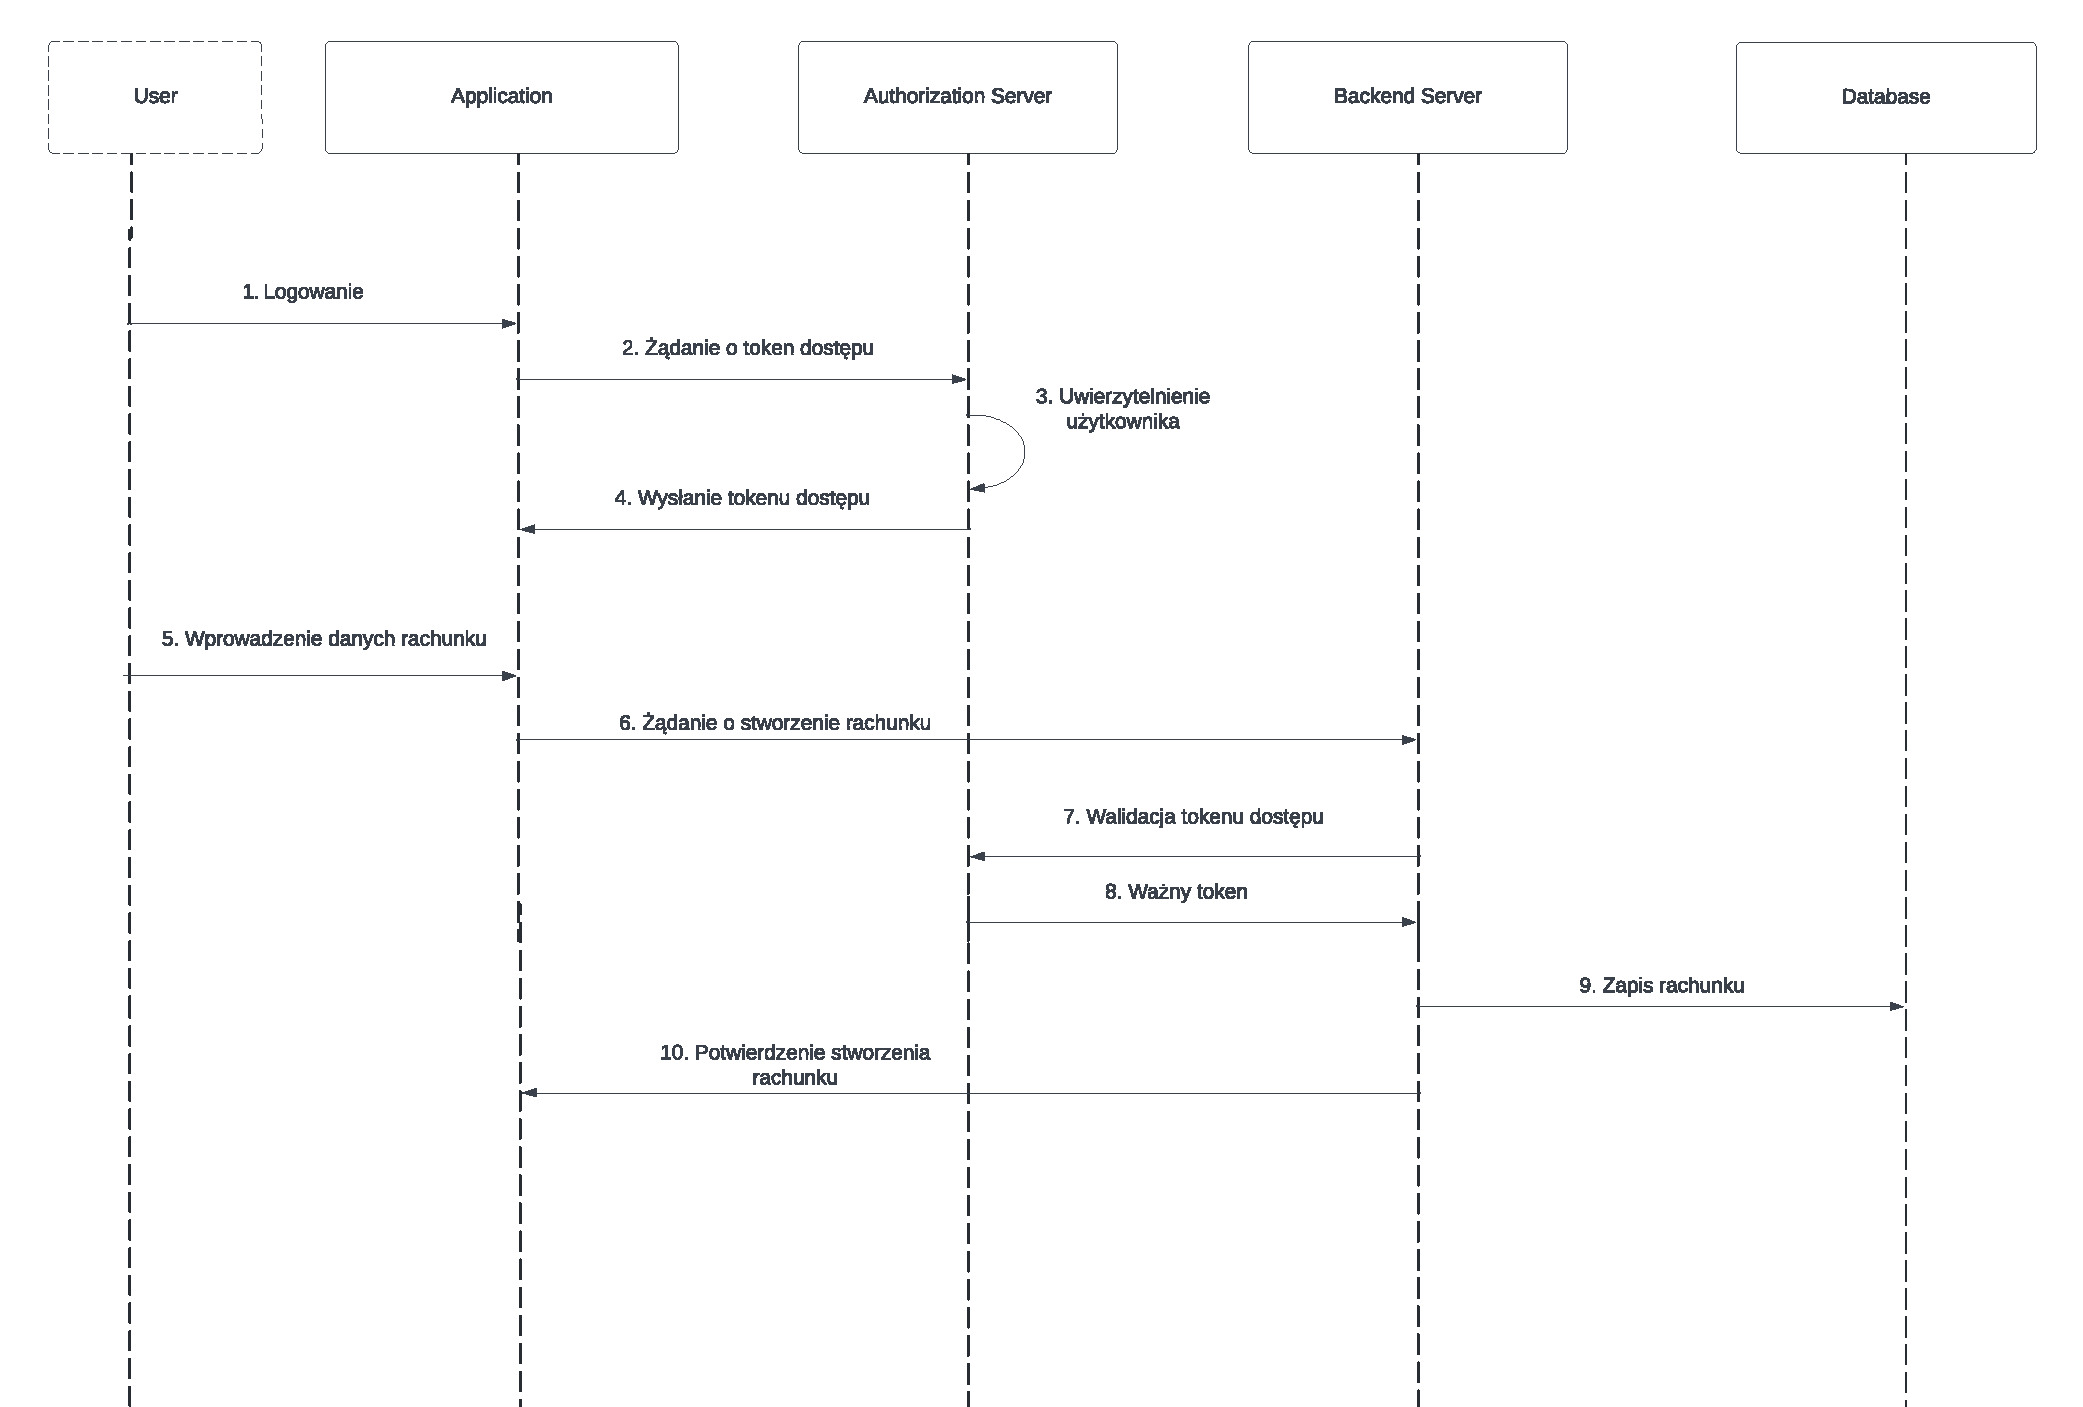
\includegraphics[width=1\textwidth]{img/Diagram sekwencji.pdf}
    \caption{Diagram sekwencji}
    \label{fig:mesh1}
\end{figure}

\section{Bezpiczeństwo}
\subsection{Zabezpieczenia logowania i autoryzacji Zarządzanie sesjami}
\begin{itemize}
    \item Technologie: OAuth 2.0
    \item Uzasadnienie: Używa ona tokenów dostępu, które są wymieniane między klientem a serwerem. Wykorzystanie tej technologii pozwala ominąć przekazywanie danych wrażliwych między klientem a serwerem, co zmniejsza ryzyko wycieku danych. OAuth 2.0 umożliwia także zarządzanie sesją użytkownika. Przy każdym żądaniu klient przesyła token dostępu, co pozwala serwerowi identyfikować użytkownika i autoryzować sesję.
\end{itemize}
\subsection{Zabezpieczenia bazy danych}
\begin{itemize}
    \item Wrażliwe dane zostaną zaszyfrowane za pomocą bcrypt (szyfrowanie haseł) i AES (szyfrowanie innych danych wrażliwych),
    \item Zabezpieczenie przed SQL injection poprzez wykorzystanie ORM zamiast surowych zapytań oraz walidacja danych wejściowych.
\end{itemize}

\subsection{Zarządzanie dostępem}
W celu zarządzania dostępem zostaną utworzone odpowiednie role, takie jak administrator i użytkownik, które będą posiadały właściwe uprawnienia i dostęp do zasobów. Przykładowo, administrator będzie miał dostęp do logów serwerowych oraz do historii wszystkich użytkowników, natomiast pojedynczy użytkownik będzie miał dostęp wyłącznie do informacji o swoim koncie.

\end{document}